% !TEX root = ../main.tex

\section{Library Bindings}
\label{sub:interfacing_with_emlib}

This section describes the different \lib{bindings} libraries that was developed as part of the {\rg} platform.
The \gls{ffi} available in {\rust} has been used to interface with Silicon Labs' suite of {\C} libraries used to control the {\gecko}.
This way, we have been able to create wrappers around the \gls{api} for the different peripherals that we have used in the project, without porting the core logic itself.
These wrappers are called language bindings.
The following sections explain the process of defining and implementing the \gls{ffi} in {\rust} that is used to access and control the peripherals on the {\gecko}.

\subsection{The Libraries}
\label{ssub:the_bindings_library}

In \autoref{sec:back:lib} we presented the three libraries that we have created partially binding support for; \gls{cmsis}, {\emlib} and {\emdrv}.
Here, we will take a closer look at which modules from these libraries that we have written bindings for, and our reasoning for choosing each one.

We have also written many example applications in {\rust} that utilize the bindings for many of the {\gecko}'s peripherals.
These examples have been a driving factor for defining new bindings.
As an example, if we were to need some functionality for the \gls{adc}, we would define these bindings alongside the development of the examples.
In this way, the bindings have been defined incrementally during the development of either the examples that demonstrate our libraries, or the applications described in \autoref{sec:impl:project:i} and \autoref{sec:impl:project:ii}.

\subsubsection{CMSIS}
\label{sub:cmsis_bindings}

Interrupt support through \gls{nvic} was the only interesting part of the \gls{cmsis} library that we have written bindings for.
Most of the examples use one or several \gls{irq} handlers for the peripheral bindings that they demonstrate.
\gls{nvic} provides utility functions for enabling and disabling the interrupt handling mechanisms of the Cortex-M3 processor.

\subsubsection{Emlib}

When we first set out to make the bindings for {\emlib}, our priority was to define a viable platform for writing rust applications, which we could use to evaluate the language on the bare-metal system.
\autoref{tab:emlib_peripheral_bindings} summarizes some modules from {\emlib} that we have written bindings for, and why we wanted these bindings.
A list of examples that demonstrates how the bindings work is shown in \autoref{tab:emlib_examples}.
These are either written from scratch, or directly ported from {\emlib}'s examples.

\begin{table}[H]
  \centering
  \begin{tabular}{r|p{10cm}}
    \textbf{Module} & \textbf{Purpose} \\
    \hline
\prog{cmu}     &
The \gls{cmu} provides functions to manage the different clocks and oscillators on the {\gecko}.
This module is necessary in order to configure the clocks that are required by other peripherals to function. \\

\prog{dma}     &
We wanted to try to use \gls{dma} for the {\tracker} application because it can be used to transfer data without using the \gls{cpu}.
This device was also used for our experiments with higher-level abstractions in \autoref{sec:rust-embedded-modules}. \\

\prog{ebi}     &
The \gls{ebi} is used to memory map external devices connected to bus on the {\gecko}.
This simplifies the process of writing data to e.g. the \gls{lcd} on the {\chip{DK}}. \\

\prog{emu}     &
The \gls{emu} module controls the different energy modes on the {\gecko}.
We needed this functionality for the {\tracker} application. \\

\prog{gpio}    &
The \gls{gpio} was one of the first modules to be ported.
It is used extensively throughout the bindings and in the applications. \\

\prog{lesense} &
The \gls{lesense} can be configured to automatically collect data from multiple sensors, which we needed for the a initial version of the {\tracker}. \\

\prog{acmp}    &
The \gls{acmp} was ported alongside \gls{lesense}, and is used to compare two analog signals and tell which one is greater. \\

\prog{adc}     &
The \gls{adc} was needed by the {\tracker}, and has been used to get the internal temperature of the \gls{cpu}. \\

\prog{usart}   &
Primarily we wanted the \gls{usart} for easy debugging and I/O from a computer. \\

\prog{leuart}  &
The \gls{leuart} was ported a while after the \gls{usart}.
It has the same functionality, but it works with a lower-frequency clock and requires less energy than the \gls{usart}. \\

\prog{i2c}     &
The \gls{i2c} protocol has many of the same use cases as the different \gls{uart} types, but it works at lower energy levels.
It is used by the {\tracker}. \\

\prog{rtc}     &
The \gls{rtc} was an easy module to write bindings for.
It is used in several examples for timing purposes, as well as in the {\tracker}. \\

\prog{timer}   &
The Timer was one of the first modules to be ported.
It worked as a proof-of-concept for the design of the bindings, as described later in this section. \\

    \hline
  \end{tabular}

  \caption{Peripheral bindings for {\emlib}.}
  \label{tab:emlib_peripheral_bindings}
\end{table}


\begin{table}[H]
  \centering
  \begin{tabular}{r|p{8cm}|c}
    \textbf{Example} & \textbf{Purpose} & \textbf{Ported} \\
    \hline
\prog{buttons\_int}  &
Demonstrates interrupts by lighting a led on the {\chip{STK}} when the respective button has been pressed. & \cmark \\

\prog{rtc\_blink}    &
Toggle a led with an interval of 2 seconds. & \cmark \\

\prog{energy\_modes} &
Demonstrates the four stages of sleep on the {\gecko}. & \cmark \\

\prog{uart}          &
Demonstrates serial communication over \gls{uart} by echoing back every byte it receives. & \cmark \\

\prog{leuart}        &
Similar example as \prog{uart}, but the \gls{cpu} is turned off and the functionality is moved to an interrupt handler instead. & \cmark \\

\prog{i2c}           &
Sends and receives a data-buffer between two devices that supports \gls{i2c}. & \cmark \\

\prog{joystick}      &
Reads analog signals generated by a Joystick that is connected to the {\chip{STK}}. & \\

{\prog{dma}}           &
Transfer a data-buffer from one memory location to another. & \cmark \\

\prog{light\_sense}  &
Uses the {\chip{STK}}'s light sensor to measure the light intensity, and lights a LED when the intensity goes below a threshold & \cmark \\

\prog{boxes}         &
Demonstrates dynamic memory allocation with \code{Box}'es, provided by the {\rust} \lib{alloc} library.  &  \\

\prog{vec}           &
Demonstrates dynamically allocated strings and vectors from the \lib{collections} library. & \\

    \hline
  \end{tabular}

  \caption{Examples that demonstrates how the bindings work.}
  \label{tab:emlib_examples}
\end{table}

A complete overview of the progress of binding {\emlib} is given in \autoref{tab:emlib:progress}.

\newcommand{\low}{\cellcolor{red!25}}
\newcommand{\medium}{\cellcolor{yellow!25}}
\newcommand{\high}{\cellcolor{green!25}}

\begin{table}[H]
  \centering
  \begin{tabular}{l | l | l | r | l | l | l | r }
    \textbf{Module} & \textbf{\#C} & \textbf{\#R} & \textbf{Ported} & \textbf{Module} & \textbf{\#C} & \textbf{\#R} & \textbf{Ported} \\

    \hline
    \texttt{acmp}    & 15 & 3  & {\low}    20.00\% & \texttt{lcd}     & 51 &  0 & {\low}     0.00\% \\
    \texttt{adc}     & 16 & 6  & {\medium} 37.50\% & \texttt{lesense} & 52 & 21 & {\medium} 40.38\% \\
    \texttt{aes}     & 19 & 0  & {\low}     0.00\% & \texttt{letimer} & 14 &  0 & {\low}     0.00\% \\
    \texttt{assert}  & 0  & 0  &            N/A    & \texttt{leuart}  & 19 & 12 & {\medium} 63.16\% \\
    \texttt{bitband} & 4  & 0  & {\low}     0.00\% & \texttt{mpu}     &  3 &  0 & {\low}     0.00\% \\
    \texttt{burtc}   & 28 & 0  & {\low}     0.00\% & \texttt{msc}     & 19 &  0 & {\low}     0.00\% \\
    \texttt{chip}    & 1  & 1  & {\high}  100.00\% & \texttt{opamp}   &  2 &  0 & {\low}     0.00\% \\
    \texttt{cmu}     & 45 & 7  & {\low}    15.56\% & \texttt{part}    &  0 &  0 &            N/A    \\
    \texttt{common}  & 0  & 0  &            N/A    & \texttt{pcnt}    & 23 &  0 & {\low}     0.00\% \\
    \texttt{dac}     & 16 & 0  & {\low}     0.00\% & \texttt{prs}     &  4 &  1 & {\medium} 25.00\% \\
    \texttt{dbg}     & 4  & 0  & {\low}     0.00\% & \texttt{rmu}     &  6 &  0 & {\low}     0.00\% \\
    \texttt{dma}     & 22 & 8  & {\medium} 36.36\% & \texttt{rtc}     & 14 & 13 & {\high}   92.86\% \\
    \texttt{ebi}     & 42 & 9  & {\low}    21.43\% & \texttt{system}  & 11 &  0 & {\low}     0.00\% \\
    \texttt{emu}     & 24 & 17 & {\medium} 70.83\% & \texttt{timer}   & 27 & 24 & {\high}   88.89\% \\
    \texttt{gpio}    & 33 & 31 & {\high}   93.94\% & \texttt{usart}   & 26 &  6 & {\low}    23.08\% \\
    \texttt{i2c}     & 17 & 6  & {\medium} 35.29\% & \texttt{vcmp}    & 29 &  0 & {\low}     0.00\% \\
    \texttt{idac}    & 0  & 0  &            N/A    & \texttt{version} &  0 &  0 &            N/A    \\
    \texttt{int}     & 2  & 2  & {\high}  100.00\% & \texttt{wdog}    &  5 &  0 & {\low}     0.00\% \\
    \hline
    &&&& \textbf{total} & 593 & 167 & {\medium}28.16\% \\
    \hline
    \multicolumn{8}{l}{\textbf{\# C} - Number of functions exposed by {\emlib}} \\
    \multicolumn{8}{l}{\textbf{\# R} - Number of functions bound by bindings} \\
  \end{tabular}
  \caption{Bindings progress for {\emlib}}
  \label{tab:emlib:progress}
\end{table}


\subsubsection{Emdrv}
\label{sub:emdrv_bindings}

As with {\emlib}, it was not a goal to fully support all available peripheral drivers that are available in \prog{emdrv}.
The drivers that we have partially implemented bindings for are summarized in \autoref{tab:emdrv_bindings}.
They are not that hard to grasp or use since they are all fairly small.
The project includes two examples that demonstrate how to use the flash driver
The examples are summarized in \autoref{tab:emdrv_examples}.

\begin{table}[H]
  \centering
  \begin{tabular}{r|p{10cm}}
    \textbf{Driver} & \textbf{Purpose} \\
    \hline

\prog{dmactrl}  &
This binding only exports one function to return a standard \emph{\gls{dma} Descriptor} which is used to initiate a \gls{dma} transfer. \\

\prog{flash}  &
The flash driver adds an abstraction layer over a flash memory, and exposes functions to \emph{initialize}, \emph{read}, \emph{write} and get the \emph{device info}.
The Driver is used by the {\tracker}. \\

\prog{gpioint}  &
This driver is ported from {\C} to {\rust}. The implementation differs slightly between the two versions, but the functionality is the same.
The reasoning for porting this driver is described in \autoref{sec:porting-gpioint}. \\

\prog{i2c}  &
This driver is used by the {\tracker} application.
It exposes functions to initialize a commonly used \gls{i2c} data transfer configuration. \\

\prog{tft}  &
This binding exposes one function to initialize the TFT screen on the {\chip{DK}}.
It is used in the {\cg}. \\

    \hline
  \end{tabular}

  \caption{Driver bindings for \prog{emdrv}.}
  \label{tab:emdrv_bindings}
\end{table}

\begin{table}[H]
  \centering
  \begin{tabular}{r|p{8cm}|c}
    \textbf{Example} & \textbf{Purpose} & \textbf{Ported} \\
    \hline

\prog{flash} &
Demonstrates reading and writing to the {\chip{STK}}'s flash memory. & \cmark \\

\prog{light\_measure} &
Based on the \prog{light\_sense} example from \autoref{tab:emlib_examples}.
The results from measuring the light intensity is saved to flash.
When the user presses a button the {\chip{STK}} will initiate a transfer that reeds all the data stored to flash and transmits it over a \gls{usart} connection. & \cmark \\

    \hline
  \end{tabular}

  \caption{Examples that demonstrate how to use the flash bindings.}
  \label{tab:emdrv_examples}
\end{table}

\subsection{Defining the Bindings}

The {\emlib} module for controlling the \code{Timer} peripheral \cite{an0014_timer} works as a good example to demonstrate what the {\rust} bindings look like.
The module is fairly small, it mostly exposes functions to set up and initialize four different timers that can be used for up, down, up/down, and input- and output-capture.
The program shown in \autoref{lst:timer_program_c} is an example of initializing the \code{Timer0} peripheral on the {\gecko}.
Note that this is not a complete working example, it only shows the most important parts required to use the Timer module.

\begin{listing}[h]
\begin{ccode}
// Select TIMER0 parameters
TIMER_Init_TypeDef timerInit = TIMER_INIT_DEFAULT;
// Enable overflow interrupt
TIMER_IntEnable(TIMER0, TIMER_IF_OF);
// Enable TIMER0 interrupt vector in NVIC
NVIC_EnableIRQ(TIMER0_IRQn);
// Set TIMER Top value
TIMER_TopSet(TIMER0, TOP);
// Configure TIMER
TIMER_Init(TIMER0, &timerInit);
\end{ccode}
\caption{Initializing a Timer in {\C}}
\label{lst:timer_program_c}
\end{listing}

First, an initialization structure for the Timer module is acquired.
This structure has fields to configure many different properties of the Timer, in the same way as described in \autoref{ssec:memory_mapped_io}.
The next lines enable interrupts for the Timer, and the \gls{nvic} interrupt vector is set up to call the function shown in \autoref{lst:timer_interrupt_handler} every time an interrupt it triggered by the Timer.
Note that this function is called implicitly by the runtime as \autoref{sec:impl:handling-interrupts} describes.
All this function does is to clear the interrupt signal and toggle the value of a LED.
We can imagine an application where the Timer is configured to trigger an interrupt every minute to toggle the LED, and in between the interrupts the \gls{mcu} can be put to sleep in order to save power.
Interrupts like this are an important part of programming the {\gecko}.
They can be used for an asynchronous programming model where the application is defined by the code in the different interrupt handlers, and like in the example above, the \gls{mcu} can be put to sleep in between interrupts.

\begin{listing}[h]
\begin{ccode}
void TIMER0_IRQHandler(void) {
  // Clear flag for TIMER0 overflow interrupt
  TIMER_IntClear(TIMER0, TIMER_IF_OF);
  // Toggle LED ON/OFF
  GPIO_PinOutToggle(LED_PORT, LED_PIN);
}
\end{ccode}
\caption{Timer interrupt handler}
\label{lst:timer_interrupt_handler}
\end{listing}

The equivalent program written in {\rust} is shown in \autoref{lst:timer_program_rust}.
Semantically, they are the same, but the usage differs slightly, which is natural since we are using a higher level programming language.
Instead of calling functions that are included through a {\C} header file, we are calling functions that are available through a {\rust} module.
For example, the \func{enable\_irq} function is part of the \code{nvic} module.
This modularization of peripherals can help to make the code less verbose by partially including modules.
It is also worth to notice the difference between how the \code{Timer0} structure can be treated like an object with its own member methods in {\rust}, instead of being passed as the first parameter to every function that requires it, like in {\C}.

\begin{listing}[h]
\begin{rustcode}
// Select TIMER0 parameters
let timer_init = Default::default();
// Enable overflow interrupt
let timer0 = timer::Timer::timer0();
timer0.int_enable(timer::TIMER_IF_OF);
// Enable TIMER0 interrupt vector in NVIC
nvic::enable_irq(nvic::IRQn::TIMER0);
// Set TIMER Top value
timer0.top_set(TOP);
// Configure TIMER
timer0.init(&timer_init);
\end{rustcode}
\caption{Initializing a Timer in {\rust}}
\label{lst:timer_program_rust}
\end{listing}

\subsection{Exposing Static Inline Functions to Rust}
\label{ssec:exposing_static_inline_functions_to_rust}

In order to work with structures and enums originally defined in {\C}, we had to redefine them in {\rust} and mark them with \attrib{\#[repr(C)]} so that {\rust} can guarantee that the data-elements are {\C} compatible.
The header files in the peripheral \gls{api} also define many functions as \code{static inline}, which only make the functions accessible to the program that includes the header file.
Since it is not possible to include {\C} header files directly in {\rust}, we had to expose these functions through one extra layer of {\C} code.
As an example, the \func{TIMER\_IntEnable} function is defined as \code{static inline} in \file{em\_timer.h}.
In order to call this function through the {\C} \gls{abi} in {\rust}, we had to expose it through the file \file{timer.c}, as shown in \autoref{lst:exposing_static_inline}.

\begin{listing}[h]
\begin{ccode}
#include "en_timer.h"

void STATIC_INLINE_TIMER_IntEnable(TIMER_TypeDef *timer,
                                   uint32_t flags) {
  TIMER_IntEnable(timer, flags);
}
\end{ccode}
\caption{Exposing a \code{static inline} function to {\rust}.}
\label{lst:exposing_static_inline}
\end{listing}

In the {\rust} module definition of Timer, the function has to be made available through an \code{extern} block, as shown in \autoref{lst:rust_ffi_example}.
As described in \autoref{ssub:unsafe_code}, every function available through the \gls{ffi} are considered {\unsafe} because {\rust} knows nothing about the function, other than its parameters and its return value.
Thus, in order to make it practical to use the library in a seemingly safe manner, we wrap the calls to the foreign functions in an {\unsafe} block in the respective function defined in {\rust}.

\begin{listing}[h]
\begin{rustcode}
impl Timer {
  pub fn int_enable(&self, flags: u32) {
    unsafe { STATIC_INLINE_TIMER_IntEnable(self, flags) }
  }
}

extern {
  fn STATIC_INLINE_TIMER_IntEnable(timer: &Timer, flags: u32);
}
\end{rustcode}
\caption{Defining and using a function through the {\rust} \gls{ffi}.}
\label{lst:rust_ffi_example}
\end{listing}

If we compare the call-stacks between calling the \code{timer0.int\_enable} function in {\rust}, and calling the \func{TIMER\_IntEnable} function in {\C}, we can see that every function call through the \gls{ffi} requires \emph{two} extra function calls.
These are simple wrappers that require extra unconditional jumps in the code, and performance-wise it is a very unnecessary overhead to have one or two extra stack frames allocated for \emph{every} function call through the \gls{ffi}.
However, this overhead can be removed completely by optimizing the code during compilation so that the {\C} code can be called with no overhead \cite{web:rust_once_run_everywhere}.
The extra function call due to the static inline wrapper on the {\C} side of the interface will be removed by a trivial function inlining, as the only contents of the wrapper is a call to the actual function.
Additionally, by enabling \gls{lto} during the compilations, LLVM will inline the {\C} implementation into the code for the \code{timer0.int\_enable} function in {\rust}.
This results in the same performance and similar call-stacks for both {\C} and {\rust}.
This is a working example of one of {\rust}'s many zero-cost abstractions, enabled through the interoperability with the {\C} \gls{abi} and exploiting features given by LLVM.

\subsection{Naming Conventions}

We have tried to keep \emlib's naming convention across the layer of bindings.
This makes it easy for anyone reading either the {\C}- or the {\rust}-code to translate and understand the code between the two languages.
Since every constant, enum-field, or struct-name is directly accessible by name in {\C}, if the corresponding header file is included, it is important that names of such fields can be separated from each other and do not cause a naming collision.

\begin{listing}[h]
\begin{ccode}
typedef enum {
  timerCCModeOff     = _TIMER_CC_CTRL_MODE_OFF,
  timerCCModeCapture = _TIMER_CC_CTRL_MODE_INPUTCAPTURE,
  // ...
} TIMER_CCMode_TypeDef;
\end{ccode}
\caption{Part of a Timer enum defined in {\C}.}
\label{lst:enum_naming_c}
\end{listing}

As an example, two fields of an enum from \file{em\_timer.h} are shown in \autoref{lst:enum_naming_c}.
From each field in the enum we can extract 1) its module name \file{timer}, 2) its typedef name \code{CCMode} and 3) its field name \code{Off} or \code{Capture}.
{\rust} allows us to keep the same naming convention at the same time as utilizing its modularity.
\autoref{lst:enum_naming_rust} shows the enum ported to {\rust}, where both the module name and the typedef name has been left out, and only the field names have remained.
However, the naming convention remains the same when the fields are used, e.g. the expression ``\code{let mode = timer::CCMode::Capture;}'' in {\rust} shows the similarity with the equivalent expression in C: ``\code{int mode = timerCCModeCapture;}''.

\begin{listing}[h]
\begin{rustcode}
pub enum CCMode {
  Off     = _TIMER_CC_CTRL_MODE_OFF,
  Capture = _TIMER_CC_CTRL_MODE_INPUTCAPTURE,
  // ...
}
\end{rustcode}
\caption{The enum ported to {\rust}.}
\label{lst:enum_naming_rust}
\end{listing}

\subsection{Testing}
\label{ssub:testing}

Verification of correctness is an important part of all software, whether it is done manually or with an automated test framework.
This section describes a small unit test framework that was developed for testing the bindings for {\emlib}.

\subsubsection{Why Unit testing}

Early on in the development phase of the {\emlib} bindings we saw the need for a testing framework.
This was provoked by the fact that testing software on an embedded system is a time consuming and tedious task.
More often than not you find yourself running the code in the debugger, inspecting the call stack and function arguments, to ensure that the bindings are calling the correct functions, with the correct arguments.
The fact about arguments has a subtle point to it.

We are working in two statically typed languages that lead the compiler to statically ensure that the correct types are passed around.
However, there are no checks to ensure that the memory layout of the datatypes in {\C} and {\rust} match at the borders between the two languages.
Currently, the {\rust} \gls{ffi} requires the programmer to redefine the {\C} datatypes in {\rust}, like structs and enums, in order to call into the {\C} functions that takes these datatypes as arguments.
The process of verifying this manually proved to be both error prone and time consuming, which suggested the need for an automated system to verify the correctness of the bindings.

\subsubsection{Framework}

To meet this problem, a lightweight testing framework was developed which enabled this verification to be automated.
The goal of the framework was to initialize the data on the {\rust} side, call functions via the \gls{ffi}, and verify that the correct functions were called with the exact data as supplied.
In order to do this, we made a framework that could replace {\emlib}'s code with statically generated test mocks, before calling these mocked functions from {\rust} and then verify that the functions where called correctly in {\C}.

The implemented framework is a small test runner that utilizes CMock\footnote{\url{http://www.throwtheswitch.org/}\label{foot:throw}} and Unity\footref{foot:throw}, for mocking and assertions, respectively.
Given a {\C} header file, the CMock library generates an \emph{mock} implementation of the interface for the module.
The test code is then compiled by linking to the mock implementation instead of the library, {\emlib} in our case.
In the test case, the mock can be configured to verify that our bindings are using the mock as expected.
All of the unit tests were compiled into a binary that was executed on the {\gecko}, which reported back via \gls{usart} whether the tests failed or ran successfully.
In addition, an easy to assess feedback was given by one LED lit for failure and two LED lit for success.

An example of what the testing looks like is shown in \autoref{lst:test:adc}.
It shows a test case that is used to verify that the \texttt{ADC\_Init} function is called with a default argument.

\begin{listing}[H]
  \centering
  \begin{minipage}{\textwidth}
  \begin{listing}[H]
    \begin{rustcode}
fn test_init_called_with_default() {
  // FFI call to the C function below
  unsafe { adc_expect_init_called_with_default(); }

  let adc0 = adc::Adc::adc0();
  // Call the emlib bindings with a default argument
  adc0.init(&Default::default());
}
    \end{rustcode}
    \caption{{\rust} side of \code{ADC\_Init} test}
    \label{lst:test:adc:rust}
  \end{listing}
  \end{minipage}

  \begin{minipage}{\textwidth}
  \begin{listing}[H]
    \begin{ccode}
void adc_expect_init_called_with_default() {
  static ADC_Init_TypeDef init = ADC_INIT_DEFAULT;
  // Set up the expected value on the Mock
  ADC_Init_Expect(ADC0, &init);
}
    \end{ccode}
    \caption{C side of \code{ADC\_Init} test}
    \label{lst:test:adc:c}
  \end{listing}
  \end{minipage}

  \caption{Test case for \code{ADC\_Init} with default values}
  \label{lst:test:adc}
\end{listing}

When using mocking in unit tests, the workflow for the user seems reversed compared to standard unit tests.
First, you set up the expected results by calling the \texttt{ADC\_Init\_Expect} function on the mock, as shown in \autoref{lst:test:adc:c}.
This method is called through \gls{ffi} right at the top of the test case in \autoref{lst:test:adc:rust}.
Then, after the expected result is set up, the test case goes on to create an \gls{adc} object by using the {\rust} bindings, and calls the \texttt{init} function that causes the \gls{ffi} library bindings to be executed.
When the test returns, the test runner is responsible for calling a \texttt{Verify} function on the mock object.
This function causes the program to fail and report its status over \gls{usart} if the expected result was not met.

\autoref{fig:test-framework} shows a diagram of the program flow between the \textit{Test Runner}, the \textit{Test Case}, the \textit{emlib bindings} as \gls{cut}, and the \textit{emlib mock}, for when the test case above is executed.
We see that the two boxes marked with \textit{Test Case} are the pieces of code the user of the framework, presented in \autoref{lst:test:adc}, writes.
The stippled vertical line shows the separation between {\rust} and {\C} code, all the three function calls which cross this line is implemented using the {\rust} \gls{ffi}.

\begin{figure}[H]
  \begin{center}
    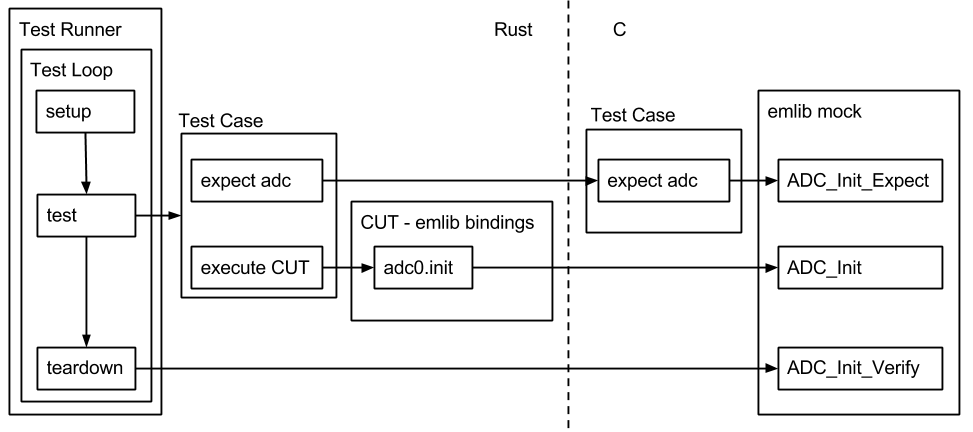
\includegraphics[scale=0.3]{figures/testframework}
  \end{center}
  \caption{Flowchart for test framework}
  \label{fig:test-framework}
\end{figure}


\subsubsection{Rust libtest}

The {\rust} programming language contains a testing framework within the standard library.
The reasons for not using it to test the bindings is that we needed to run the tests on the {\gecko}.
The rationale for this is that the tests are mostly checking that the datatypes used on the {\rust} and {\C} side of the bindings are compatible.
Therefore we need to use the proper compilers and compile the test targets for the ARM platform.
Verifying that the platform-specific \prog{gcc} and {\rustc} have compatible types does not help in respect to this.
Consequently, {\rust}'s standard testing framework relies heavily on {\rust}'s own {\std} library, which renders the framework unusable for our bare-metal platform.

% Consequently, {\rust}'s standard testing framework is rendered unusable for our embedded platform because it relies heavily on the {\rust}'s own {\std} library.

% Consequently, given that the testing framework in the standard library relies heavily on the  that was discussed in \autoref{sec:back:lib}, this renders the framework unusable for our embedded platform.

\subsection{Discussion}

Writing the bindings for the different peripherals was a tedious work, that required careful review of the {\emlib} source code in order to correctly port enum- and struct-definitions from {\C} to {\rust}.
Additionally, we had to redefine many constants, like the names of memory-mapped register bit-fields like the ones presented earlier in \autoref{fig:back:memorymapped}, or values calculated from various {\C} macros defined in header files that are used throughout the library.
If they were only implicitly defined in the header files, we had to retrieve the value of the constants by debugging the source code and explicitly look up the value of these constants.

Since we have constrained our library to only support the Giant Gecko devices, we chose to manually write the bindings for the library instead of generating the bindings through some kind of automated process.
There were already a couple of tools available for generating such {\C}-bindings automatically, that could possibly have made the process quicker.
However, we chose not to utilize such tools because of the reasons described below.

\begin{itemize}
    \item It was quick and easy to get started with code for a new peripheral.
    This argument was especially important when the project started out, because we still had no clue of how the project would evolve and what it was going to look like.

    \item It was an advantage to depend on as few third party tools as possible, since both {\rust} and all available libraries would be unstable until the 1.0 release of the language.

    \item We wanted to keep the naming convention of our bindings as similar to {\emlib} as possible.
    This would not have been easy to keep consistent with an automated process, partly because there are exceptions where these conventions do not fully hold.
    It is however an interesting problem that would have a higher priority if the library were ever to support more than one EFM32 device.

    \item We could focus on writing bindings for smaller parts of each module separately when we first needed them, which would split the work into smaller work-packages.
\end{itemize}
